\documentclass[11pt,a4paper]{article}
\usepackage[T1]{fontenc}
\usepackage[utf8]{inputenc}
\usepackage{lmodern,amsmath,amssymb,amsthm,mathtools,booktabs,graphicx,xcolor}
\usepackage[margin=25mm]{geometry}
\usepackage{microtype,fancyhdr}
\usepackage[colorlinks=true,linkcolor=blue!45!black,urlcolor=blue!45!black,citecolor=blue!45!black]{hyperref}
\hypersetup{pdftitle={Dissipation from three observations},pdfauthor={ChatGPT},pdfsubject={Mathematical research record with proofs and synthetic validation}}
\setlength{\parindent}{0pt}\setlength{\parskip}{5pt}\setlength{\headheight}{14pt}
\pagestyle{fancy}\fancyhf{}
\fancyhead[L]{\small Dissipation from reflected observations}
\fancyhead[R]{\small Research record, 5 November 2026}\fancyfoot[C]{\thepage}
\newtheorem{theorem}{Theorem}
\newtheorem{proposition}[theorem]{Proposition}
\newcommand{\E}{\mathbb E}\newcommand{\Prb}{\mathbb P}
\newcommand{\one}{\mathbf 1}\newcommand{\KL}{D_{\mathrm{KL}}}
\newcommand{\TV}{\operatorname{TV}}\newcommand{\atanh}{\operatorname{artanh}}
\newcommand{\tr}{\operatorname{tr}}
\title{Dissipation from three observations\\\large Reflection bounds beyond pair correlations and the visible arrow of time}
\author{Independent research conducted with ChatGPT}
\date{5 November 2026}
\begin{document}
\maketitle
\begin{abstract}
We ask whether sparse observations can impose a positive thermodynamic cost on every compatible hidden Markov architecture, even when all two-time laws admit an equilibrium explanation and the entire visible process is time-reversal symmetric. Within stationary finite continuous-time Markov models whose microscopic states are even under physical reversal, the answer is yes.

For a bounded score $g$ on a half-record of duration $t$, with range $R$, and central weight $0\leq w\leq1$, write $C=\E[w g_-g_+]$. We prove $\sigma\geq8[-C]_+/(R^2t)$ and a nonlinear refinement. A four-state construction has exactly the pair laws of an equilibrium telegraph process and a completely reversible visible path law, while its three-observation conditional covariance is negative. Four states are minimal for this exact separation. We give a matrix generalization, a stationary single-record equilibrium test requiring no mixing bound, a conservative rate confidence interval without mixing, and a stronger protocol with paid preparation and decorrelation. Synthetic calculations verify the construction and execute the protocols.

\textbf{Status.} These are internally derived mathematical results with numerical checks. Time-symmetric hidden dissipation and the qualitative reflection principle are prior work. The candidate contribution is the quantitative refinement and completed sparse-observation construction and inference chain. The bounded literature audit does not establish priority. This report does not establish a civilization-changing discovery or a laboratory demonstration.
\end{abstract}
\setcounter{tocdepth}{1}
\begingroup\small\setlength{\parskip}{0pt}
\tableofcontents
\endgroup
\newpage
\section{Question, consequence, and physical model}
An observer sees a label $Y_t$, possibly one bit, instead of the complete microscopic state. Two familiar descriptions of a recording are all its two-time statistics and its forward-versus-backward path asymmetry. We construct a family where both descriptions are exactly compatible with equilibrium, yet three observations exclude every equilibrium hidden-state explanation in a specified class.

The achieved operation is a quantitative certificate from sparse measurements. It requires neither reconstruction of the hidden graph nor a bound on its number of states. The organizing fact is that the reflected past and future of an equilibrium Markov process, conditional on the complete present state, are independent copies. Their positivity constraints are stronger than visible time symmetry. Comparing conditional forward and reverse laws directly gives a bound linear in a violated constraint.

Let $X_t$ be a stationary finite irreducible continuous-time Markov chain (CTMC), in row-generator convention, with generator $Q$ and positive stationary distribution $\pi$. Observe a deterministic finite-alphabet label $Y_t=h(X_t)$ without perturbing the dynamics. All microscopic states are \emph{even under physical time reversal}. The reverse generator is
\[
Q^*=D_\pi^{-1}Q^{\mathsf T}D_\pi,\qquad D_\pi=\operatorname{diag}(\pi).
\]
Stationarity makes $Q,Q^*$ have the same escape rate at every state. In units $k_B=1$, define
\begin{equation}\label{eq:sigma}
\sigma=\sum_{i<j}(\pi_iq_{ij}-\pi_jq_{ji})\log\frac{\pi_iq_{ij}}{\pi_jq_{ji}}.
\end{equation}
We prove the finite-$\sigma$ case, hence bidirectional support. An unpaired positive flux gives infinite $\sigma$, making the bounds automatic. This quantity is a path irreversibility rate. Identifying it with physical entropy production requires local detailed balance. Physical entropy production is then $k_B\sigma$, and steady isothermal dissipation power is $k_BT\sigma$ under that thermodynamic model.

No bound on dimension, topology, rates, or mixing enters the population inequalities. Stationarity, physical parity, and noninvasive access are substantive premises. Statistical protocols below state their extra assumptions separately.

\section{A direct reflection inequality}
Fix $t>0$. Apply the same bounded real function $g$ to the future half-record and the past read outward from the present:
\[
g_+=g((Y_s)_{0\leq s\leq t}),\qquad g_-=g((Y_{-s})_{0\leq s\leq t}).
\]
The function can use finitely many snapshots. Write $R=\sup g-\inf g>0$, $w=w(Y_0)\in[0,1]$, $C=\E[w g_-g_+]$, and $p=\E w$.
\begin{theorem}[Quantitative reflection bound]\label{thm:scalar}
For the model above,
\begin{equation}\label{eq:linear}
\boxed{\displaystyle\sigma\geq\frac{8[-C]_+}{R^2t}.}
\end{equation}
If $C<0$, set $\eta=4(-C)/(pR^2)$. Necessarily $0<\eta\leq1$, and
\begin{equation}\label{eq:nonlinear}
\boxed{\displaystyle\sigma\geq\frac{2p}{t}\sqrt\eta\,\atanh\sqrt\eta.}
\end{equation}
The right side is infinite at $\eta=1$. Equilibrium implies $C\geq0$ for every such score.
\end{theorem}
\begin{proof}
Let $P_i,P_i^*$ be hidden future half-path laws started at $i$ under $Q,Q^*$. Put $u_i=\E_{P_i}g$, $v_i=\E_{P_i^*}g$. Given $X_0=i$, the stationary past has law $P_i^*$ and is independent of the future. Therefore
\[
C=\sum_i\pi_iw_iu_iv_i\geq-\frac14\sum_i\pi_iw_i(u_i-v_i)^2.
\]
An observable of range $R$ has expectation difference at most $R\TV(P_i,P_i^*)$. Pinsker gives
\[
(u_i-v_i)^2\leq\frac{R^2}{2}\KL(P_i\Vert P_i^*).
\]
The two hidden path laws have identical initial state and escape rates. The CTMC likelihood formula averaged over $\pi$ gives exactly
\begin{equation}\label{eq:pathKL}
\sum_i\pi_i\KL(P_i\Vert P_i^*)=t\sigma.
\end{equation}
Dropping $w_i\leq1$ proves~\eqref{eq:linear}.

For the refinement let $v_i^{\rm TV}=\TV(P_i,P_i^*)$. Binary data processing gives, for any probability laws with total variation $v$,
\[
\KL(P\Vert Q)+\KL(Q\Vert P)\geq4v\atanh v.
\]
For fixed difference $v$ of Bernoulli parameters, their Jeffreys divergence is minimized at $(1\pm v)/2$, proving the inequality. Both averaged KL directions in~\eqref{eq:pathKL} equal $t\sigma$, and
\[
\sum_i\pi_iw_i(v_i^{\rm TV})^2\geq4(-C)/R^2=p\eta.
\]
The function $H(s)=\sqrt{s}\atanh\sqrt{s}=\sum_{n\geq1}s^n/(2n-1)$ is increasing and convex. Jensen with weights $\pi_iw_i/p$ proves~\eqref{eq:nonlinear}. Since $H(s)\geq s$, it includes~\eqref{eq:linear}.
\end{proof}
The hidden conditional laws are proof devices; evaluating $C$ only requires observed data. A negative score is possible even when the visible path has no arrow. Additive shifts of $g$ are allowed and can expose a stronger violation.

\section{An exact four-state separation}
Let $a>0$, $0<\epsilon<a/2$, and
\[
f=(1,1,-1,-1)^{\mathsf T},\quad h=(1,-1,1,-1)^{\mathsf T},\quad
k=f\odot h=(1,-1,-1,1)^{\mathsf T}.
\]
Define
\begin{equation}\label{eq:Q}
Q=-a(I-\one\one^{\mathsf T}/4)+\frac\epsilon4(hf^{\mathsf T}+fk^{\mathsf T}).
\end{equation}
In entries,
\[Q=\frac14\begin{pmatrix}
-3a+2\epsilon&a&a-2\epsilon&a\\
a&-3a-2\epsilon&a&a+2\epsilon\\
a&a+2\epsilon&-3a&a-2\epsilon\\
a-2\epsilon&a&a+2\epsilon&-3a
\end{pmatrix}.\]
All off-diagonal rates are positive. Rows and columns sum to zero, so $\pi_i=1/4$. Observe $Y_t=f(X_t)$.
\subsection{Every two-time law is an equilibrium law}
The centered basis satisfies $Qf=-af+\epsilon h$, $Qh=-ah$, $Qk=-ak+\epsilon f$. Thus $e^{tQ}f=e^{-at}(f+\epsilon th)$ and
\begin{equation}\label{eq:pair}
\E[Y_0Y_t]=e^{-at},\qquad\Prb(Y_0=u,Y_t=v)=\frac{1+uv e^{-at}}4.
\end{equation}
At every lag these are exactly the pair laws of an equilibrium telegraph process with flip rate $a/2$. Every function of a binary state is affine in that state, so this covers all one-time statistics and every two-time correlation of observed state functions.

\subsection{The entire visible path is time-reversal symmetric}
Let $\mathsf R$ swap hidden states 3 and 4. Then
\[
Q^{\mathsf T}=\mathsf RQ\mathsf R,\qquad\mathsf Rf=f,\qquad\mathsf R\one=\one.
\]
Each observation projector commutes with $\mathsf R$. Transpose the stationary matrix-product probability of any word, including arbitrary unequal gaps. Cancel all adjacent $\mathsf R$ factors. The result is exactly the probability of the reversed word with reversed gaps. All visible finite-dimensional laws, and consequently the visible path law, are reversible. Its forward-versus-reverse path KL is zero on every finite window.

\subsection{Three observations nevertheless exclude equilibrium}
Set $r=e^{-at}$ and $m=r^2(\epsilon t)^2$. For $u,v,z\in\{-1,+1\}$,
\begin{equation}\label{eq:triple}
\Prb(Y_{-t}=u,Y_0=v,Y_t=z)
=\frac{1+r(uv+vz)+r^2uz+muvz}{8}.
\end{equation}
One verifies its extra term from $\E[Y_0Y_sY_{s+t}]=\epsilon^2st e^{-a(s+t)}$. In particular,
\begin{equation}\label{eq:cov}
\operatorname{Cov}(Y_{-t},Y_t\mid Y_0=-1)=-\epsilon^2t^2e^{-2at}<0.
\end{equation}
For an equilibrium hidden Markov model this conditional covariance must be nonnegative: given the full center state the two sides are independent copies, so forgetting the center state gives a variance.

Choose $g(y)=y+r$, $w(y)=\one\{y=-1\}$. Then $R=2$, $p=1/2$, $C=-m/2$, and
\begin{equation}\label{eq:familybound}
\boxed{\displaystyle\sigma\geq\epsilon^2t e^{-2at}},\qquad
\sigma\geq\epsilon e^{-at}\atanh(\epsilon t e^{-at}).
\end{equation}
The linear floor is maximized at $t=1/(2a)$, giving $\sigma\geq\epsilon^2/(2ae)$. The actual rate of this realization is
\begin{equation}\label{eq:actual}
\sigma(Q)=\frac\epsilon2\log\frac{a+2\epsilon}{a-2\epsilon}
=\frac{2\epsilon^2}{a}+O(\epsilon^4/a^3).
\end{equation}
Near equilibrium the optimized linear certificate retains a fraction $1/(4e)\simeq9.20\%$. It applies to \emph{every} compatible all-even finite hidden realization, however large, rather than only to~\eqref{eq:Q}.

For $a=1$, $\epsilon=0.4$, $t=0.5$:
\begin{center}\begin{tabular}{lr}\toprule
Quantity&Value\\\midrule
Pair correlation&0.60653066\\
Conditional covariance&$-0.01471518$\\
Weighted score&$-0.00735759$\\
Linear rate floor&0.02943036\\
Nonlinear rate floor&0.02957600\\
Actual entropy production&0.43944492\\\bottomrule
\end{tabular}\end{center}

\begin{proposition}[Minimality for this exact separation]
With at most three hidden states, a stationary CTMC with a nonconstant binary observation and a single-exponential autocovariance has a two-state Markov observed process. Four hidden states are therefore minimal for the exact telegraph-pair/non-Markov separation above.
\end{proposition}
\begin{proof}
Center and normalize the binary observable. The mean-zero observable space has dimension at most two. In an orthonormal basis starting with $f$, the restricted generator is $A=\left(\begin{smallmatrix}-a&b\\c&d\end{smallmatrix}\right)$. The first derivative of the autocorrelation fixes $A_{11}=-a$; the second gives $(A^2)_{11}=a^2+bc=a^2$, hence $bc=0$. Thus $f$ is an eigenvector of $Q$ or of its stationary adjoint $Q^*$. A two-valued eigenfunction forces constant total transition rates between observation blocks (strong lumpability). If the reverse is lumpable, its stationary time reverse is Markov as well. The one-dimensional case is immediate.
\end{proof}

\begin{figure}[t]\centering
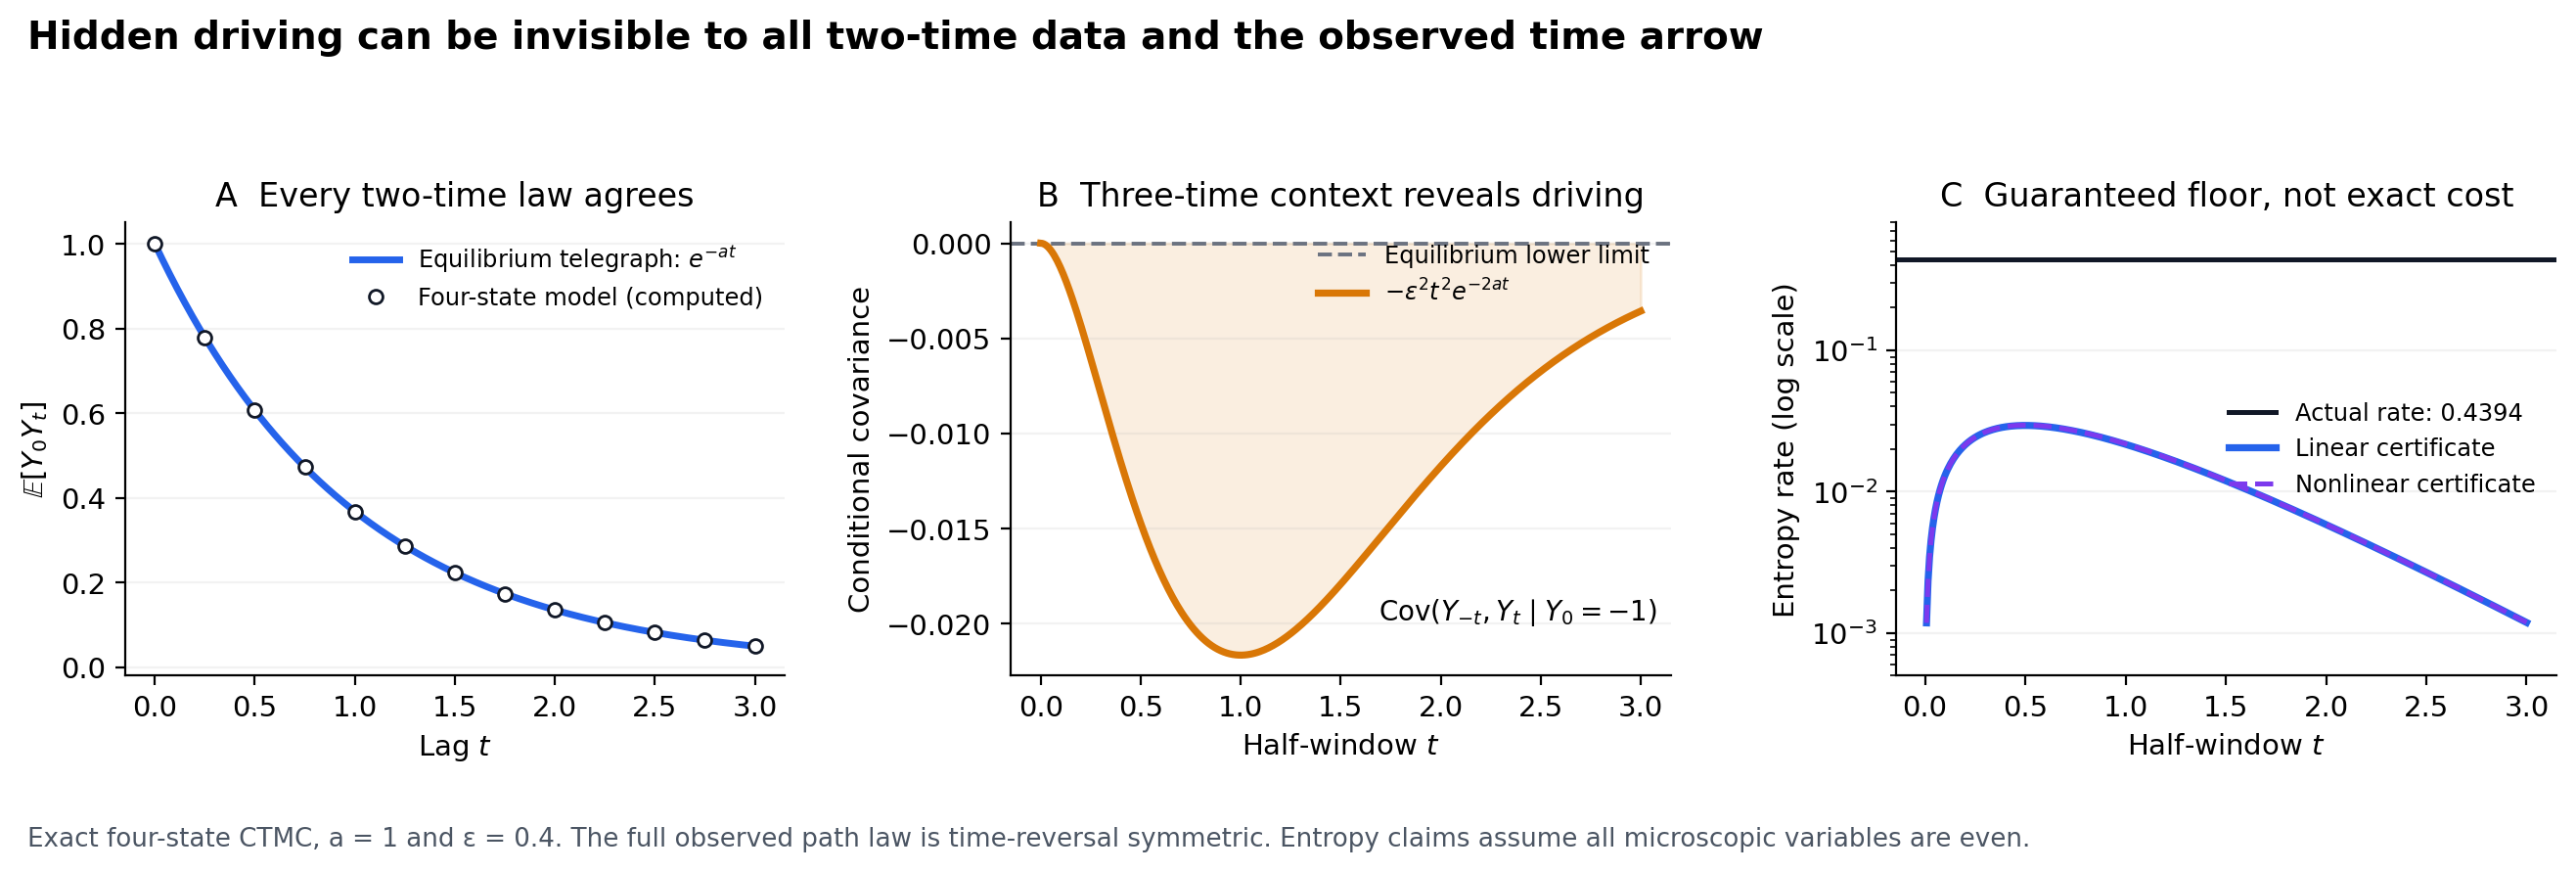
\includegraphics[width=\textwidth]{reflection_results.png}
\caption{Exact-model calculations: equilibrium two-time statistics coexist with a negative conditional three-time covariance. A positive dissipation floor follows within the all-even class. The figure is synthetic, not experimental data.}
\end{figure}

\section{A matrix representation of the obstruction}
Let $U,V$ be future and reflected-past words in half-windows of duration $t$, taking $k$ values. Put $M_{ab}=\Prb(V=a,U=b)$ and $S=(M+M^{\mathsf T})/2$. Given $X_0=i$, write their distributions $u_i,v_i\in\Delta_k$, and set $c_i=(u_i+v_i)/2$, $d_i=(u_i-v_i)/2$. Then
\begin{equation}\label{eq:matrix}
S=\underbrace{\sum_i\pi_i c_ic_i^{\mathsf T}}_{B}
-\underbrace{\sum_i\pi_i d_id_i^{\mathsf T}}_{Z}.
\end{equation}
$B$ is completely positive (a sum of outer products of nonnegative vectors); $Z\succeq0$ and $Z\one=0$. This matrix terminology is distinct from complete positivity of quantum channels. Since
\[
\|d_i\|_2^2\leq\TV(u_i,v_i)^2/2\leq\KL(u_i\Vert v_i)/4,
\]
data processing gives $\tr Z\leq t\sigma/4$. Let $r=S\one$, $A=S-rr^{\mathsf T}$, and let $\nu=\tr A_-$ be the sum of the absolute values of the negative eigenvalues of $A$. The covariance of $c_i$ is PSD, so $A+Z\succeq0$. It follows that
\[
\boxed{\displaystyle\sigma\geq\frac{4\nu}{t}},\qquad
\sigma\geq\frac2t\sqrt{2\nu}\atanh\sqrt{2\nu},\quad0\leq\nu\leq\tfrac12.
\]
The negative part is the minimum-trace PSD correction making $A$ PSD. Equivalently, with $Z\one=0$, the condition $S+Z\succeq0$ is equivalent to $A+Z\succeq0$ by the Schur complement. The nonlinear bound follows from the symmetric-divergence proof applied to the total variation distances and Jensen.

Requiring $S+Z$ to be completely positive can tighten the optimization. It is a necessary condition, not a characterization of all reversible CTMC realizations. Full word tables have $k^2$ entries. Validating a chosen scalar score avoids estimating the entire table, but finding a useful score may still be expensive.

\section{A single-record equilibrium test without a mixing bound}
Population expectations do not justify treating consecutive triples as independent. A separate theorem handles dependence under the null. Fix $g,w,t,n$ in advance, with $|g|\leq G$, $0\leq w\leq1$. Here $g$ is a function of an observed endpoint. On one stationary trajectory take adjacent blocks sharing their boundary samples:
\[
Z_r=w(Y_{(2r-1)t})g(Y_{(2r-2)t})g(Y_{2rt}),\quad
\overline Z=\frac1n\sum_{r=1}^nZ_r,\qquad B=G^2.
\]
\begin{theorem}[Uniform equilibrium rejection]\label{thm:null}
Every stationary all-even reversible hidden CTMC satisfies
\begin{equation}\label{eq:nulltail}
\Prb(\overline Z\leq-z)\leq
\exp\left[-n\operatorname{kl}\left(\frac{1+z/B}{2}\middle\Vert\frac12\right)\right]
\leq\exp\left[-\frac{nz^2}{2B^2}\right]
\end{equation}
for $0\leq z\leq B$. No hidden-dimension or mixing-time bound is used. There are $2n+1$ readings over duration $2nt$, following stationary preparation.
\end{theorem}
\begin{proof}
In $L^2(\pi)$, $P=e^{tQ}$ is self-adjoint under the null. Let $D_f$ denote multiplication by a state function. The tilted block kernel is
\[
K_\theta(i,k)=\sum_jP(i,j)P(j,k)e^{-\theta w_jg_ig_k}
=\sum_{m\geq0}\frac{(-\theta)^m}{m!}
 [D_{g^m}PD_{w^m}PD_{g^m}]_{ik}.
\]
Every bracketed coefficient is PSD and has operator norm at most $B^m$. Dropping negative odd terms yields $K_\theta\preceq\cosh(\theta B)I$. The kernel is entrywise nonnegative and self-adjoint, so Perron--Frobenius bounds absolute eigenvalues by its largest eigenvalue. $K_\theta$ need not itself be PSD. Therefore
\[
\E_\pi e^{-\theta\sum_rZ_r}=\langle\one,K_\theta^n\one\rangle_\pi
\leq\cosh(\theta B)^n.
\]
Chernoff optimization gives the binary-KL bound, while $\log\cosh x\leq x^2/2$ gives the simpler bound.
\end{proof}
A predetermined finite set of $J$ scores can be tested with budgets $\alpha/J$. Arbitrary score fitting on the same dependent record is not justified by the fixed-test result. A predefined sequence of sample sizes with summable failure budgets permits repeated checking; unrestricted optional stopping is not claimed.

\subsection{A conservative rate confidence bound without mixing}
Write $T=2t$ and $q(z)$ for the first exponential in~\eqref{eq:nulltail}. For confidence failure $\delta$, define
\begin{equation}\label{eq:nomixCI}
L_\delta(z)=\begin{cases}
\displaystyle\frac4{nT}\operatorname{kl}(\delta\Vert q(z)),&q(z)<\delta,\\[3pt]
0,&q(z)\geq\delta.
\end{cases}
\end{equation}
Then every stationary all-even CTMC, including driven ones, satisfies
\[
\Prb\{L_\delta([-\overline Z]_+)>\sigma\}\leq\delta.
\]
Its additive reversibilization $Q_s=(Q+Q^*)/2$ has the same stationary distribution and
\[
\KL(\mathcal P_Q^{[0,nT]}\Vert\mathcal P_{Q_s}^{[0,nT]})\leq nT\sigma/4.
\]
For the event $\overline Z\leq-z$, let its probabilities be $p_Q,p_s$. Data processing gives $\operatorname{kl}(p_Q\Vert p_s)\leq nT\sigma/4$ and $p_s\leq q(z)$. When $q(z)<\delta$ and $\operatorname{kl}(\delta\Vert q(z))>nT\sigma/4$, monotonicity implies $p_Q<\delta$. Threshold inversion proves the claim.

The reversibilization comparison follows edge by edge from
\[
x\log\frac{2x}{x+y}+y\log\frac{2y}{x+y}
\leq\frac14(x-y)\log\frac xy.
\]
For a proof put $v=(x-y)/(x+y)$. Differentiating the difference reduces to $2v/(1-v^2)\geq\log[(1+v)/(1-v)]$ for $0\leq v<1$.

This confidence interval is conservative: at fixed nonzero $z$, its large-$n$ floor is $4\delta I(z/B)/T$, with $I(x)=\operatorname{kl}((1+x)/2\Vert1/2)$. It does not consistently recover the full dissipation rate. Stationary initialization remains essential.

\section{Preparation, validation, and full observation costs}
For a stronger quantitative certificate from an initially arbitrary apparatus, assume a supplied uniform mixing envelope
\[
\sup_x\TV(P_s(x,\cdot),\pi)\leq e^{-\kappa s},\qquad\kappa>0.
\]
This is extra physical knowledge: visible pair correlations cannot certify it. Choose a bounded score from training data, then freeze it. Before every length-$T$ validation block, including the first, wait
\[
g=\kappa^{-1}\log\frac{8(N+M)}\delta,
\]
where $N$ is the validation count and $M$ the training count. Sequential coupling compares these blocks to independent stationary blocks, independent of training, with total failure at most $\delta/8$. The argument works for arbitrary initial states and makes no hidden-state reset.

For the binary family use a trained center $c\in[0,1]$ and
\[
H=\one\{Y_0=-1\}(Y_{-t}+c)(Y_t+c).
\]
Its range width is $W=2(1+c)$. From its held-out mean $\widehat C$, define
\[
\gamma_L=\left[-\widehat C-W\sqrt{\frac{\log(4/\delta)}{2N}}\right]_+.
\]
Then, with the stated confidence budget, $\sigma\geq2\gamma_L/t$. Let $p_U$ be an upper confidence bound on $\Prb(Y_0=-1)$. Substituting $p_U$ and $\eta_L=\gamma_L/p_U$ in~\eqref{eq:nonlinear} is conservative: for fixed $c_0$, $pH(c_0/p)$ decreases with $p$.

There are $O(N)$ score evaluations, constant working storage for a fixed score, three readings per validation block, and modeled physical duration $N(T+g)$ plus training. The detector's energy cost is not specified by this abstract access model; no claim of energetic efficiency follows. Finding a general word score can cost much more than validating one.

\subsection{Executed synthetic protocols}
The code generated one four-state trajectory with $a=1$, $\epsilon=0.4$, validation lag $t=1$, and an arbitrary initial state. It used $20{,}000$ training blocks and $750{,}000$ validation blocks. The envelope $\kappa=a-2\epsilon=0.2$ is rigorous: subtracting the uniform-refresh generator $\kappa(\one\one^{\mathsf T}/4-I)$ from $Q$ leaves a valid Markov generator.
\begin{center}\begin{tabular}{lr}\toprule
Executed quantity&Value\\\midrule
Trained center&0.3707\\
Exact pair correlation&0.36787944\\
Held-out score&$-0.00938689$\\
Hoeffding radius&0.00468559\\
95\% linear rate lower bound&0.00940259\\
95\% nonlinear rate lower bound&0.00943212\\
True generating rate&0.43944492\\
Binary readings&2,290,000\\
Gap before each block&93.1466\\
Total modeled duration&73,242,880.5\\\bottomrule
\end{tabular}\end{center}
This deliberately conservative waiting cost is not hidden behind CPU runtime.

A second run used exact uniform stationary preparation for this known four-state example, a prespecified center $c=0.37$, and $750{,}000$ consecutive length-2 blocks. It required no thinning and no mixing input to its test. It produced
\[
\overline Z=-0.01041134,\qquad
\Prb_{\rm any\ equilibrium}(\overline Z\leq-0.01041134)
\leq9.7436\times10^{-6}.
\]
It used $1{,}500{,}001$ binary readings over $1{,}500{,}000$ time units. Its conservative 95\% rate bound~\eqref{eq:nomixCI} was $1.0092\times10^{-6}$. This small bound illustrates the distinction between rejecting equilibrium and accurately bounding the stationary mean rate without a concentration assumption. Both runs are synthetic; neither is physical experimental evidence.

\section{Weak-driving sample complexity and alternative power}
For independent triples at fixed lag, the sample dependence can be matched. Let $P_\epsilon$ be~\eqref{eq:triple} and $P_0$ the equilibrium telegraph triple law. Then
\begin{equation}\label{eq:chi}
\chi^2(P_\epsilon\Vert P_0)=\frac{m^2}{(1-r^2)^2},\qquad
m=r^2(\epsilon t)^2.
\end{equation}
Indeed $P_\epsilon-P_0=muvz/8$, while $P_0=(1+ruv)(1+rvz)/8$; summing the eight reciprocals gives~\eqref{eq:chi}. Since $\KL\leq\chi^2$, a decision with both errors at most $\delta<1/2$ needs
\[
N\geq\frac{(1-r^2)^2}{m^2}(1-2\delta)
       \log\frac{1-\delta}{\delta}.
\]
This follows by data processing to the binary test decision. At fixed $a,t$, it is $\Omega(\epsilon^{-4}\log(1/\delta))$. Bounded-score validation attains this order with independent triples, since the signal is $\Theta(\epsilon^2)$.

This is an access-specific lower bound, not a lower bound for every continuously observed or adaptively timed experiment. Preparation has its own cost. Centering is comparatively cheap: the exact score is
\[
C(c)=\tfrac12\{(c-r)^2-m\}.
\]
An $O(\epsilon)$ centering error therefore suffices; estimating the pair correlation to that accuracy needs only $O(\epsilon^{-2})$ independent training samples at fixed $a,t$.

\subsection{Power of the uninterrupted test on the constructed family}
The null theorem controls false positives without a mixing input. A power statement requires separate information about the alternative. For~\eqref{eq:Q}, the uniform refresh proves contraction of the length-$T$ boundary chain by $b=e^{-\kappa T}$. Let the block score have width $W$, stationary mean $C=-\gamma$, and set
\[
L=W\left(1+\frac1{1-b}\right).
\]
For any starting state, a Doob martingale over successive block paths gives, with probability at least $1-\beta$,
\begin{equation}\label{eq:power}
\overline Z\leq-\gamma+\frac{W}{n(1-b)}
       +L\sqrt{\frac{\log(1/\beta)}{2n}}.
\end{equation}
To verify the constants, write the conditional expected future reward as a value function. The span of the remaining value is at most $W\sum_{j\geq0}b^j=W/(1-b)$, so one exposed block has martingale range at most $L$. The difference between the expected total from a fixed start and the stationary total is at most $W/(1-b)$. Conditional Hoeffding proves~\eqref{eq:power}.

Combining~\eqref{eq:power} with the null threshold $B\sqrt{2\log(1/\alpha)/n}$ yields an explicit sufficient $n$ for power $1-\beta$. For the correctly centered score $g(y)=y+e^{-at}$, at $t=\Theta(1/a)$ and $\epsilon/a\to0$, $b$ stays bounded below one and $\gamma=\Theta((\epsilon/a)^2)$. Thus $n=O((a/\epsilon)^4\log(1/(\alpha\beta)))$ suffices on a stationary uninterrupted record. This is a proved power law for this family, not a uniform power guarantee over unknown slow alternatives. Null validity still requires stationary initialization.

\subsection{Known independent readout errors}
Suppose each reading flips independently with known probability $\nu<1/2$, with $\rho=1-2\nu$. For noisy values $Z_-,Z_0,Z_+$,
\[
\widetilde H=\frac{1-Z_0/\rho}{2}
       (Z_-/\rho+c)(Z_+/\rho+c)
\]
is unbiased for the true score. The central factor may be negative; this is an estimator correction, not the nonnegative physical weight in the theorem. Its exact range follows from eight outcomes, with coarse bound
\[
|\widetilde H|\leq\tfrac12(1+\rho^{-1})(\rho^{-1}+|c|)^2.
\]
The paid-mixing validation protocol therefore tolerates a fixed calibrated flip rate, with conservative $O(\rho^{-6})$ sample penalty. At $\nu=0.1$, the executed exact-table unbiasedness error was below $5\times10^{-17}$. This corollary does not cover correlated readout memory, drift, or backaction. The nonnegative-weight no-mixing null proof must not be applied unchanged to this inverse-corrected statistic.

\section{Primary literature and exact contribution boundary}
The qualitative conditional-square/reflection principle is established mathematics, including Markov reflection positivity~\cite{reflection}. Skinner and Dunkel already obtained positive dissipation bounds for fully time-symmetric observations by optimization over hidden mechanisms~\cite{sd_pnas}. Their waiting-time method is another strong comparator~\cite{sd_prl}. These phenomena are not discoveries of this report.

The public, unrefereed October 2026 candidate on architecture-independent dissipation~\cite{floor} already uses negative reflected persistence correlations and additive reversibilization to obtain hidden-dimension-independent bounds. We inspected its manuscript and source audit. Its exact-law classification concerns alternating-renewal observations. The potential increment here is the direct $Q$-versus-$Q^*$ inequality, linear in the negative reflection defect; the general bounded-score and matrix form; and the completed finite-snapshot construction and statistical procedure. Tilted-operator concentration and uniform hidden-equilibrium testing also have methodological antecedents; they are not claimed as entirely new ideas.

Richer waiting-time information detects our example too. Its mean dwell is $2/a$ in both labels, while
\[
\mathrm{CV}_+^2=\frac{2a^2+\epsilon^2}{2a^2-\epsilon^2}>1,
\qquad
\mathrm{CV}_-^2=\frac{2a^2-\epsilon^2}{2a^2+\epsilon^2}<1.
\]
Thus there is no claimed advantage over optimal full-record or continuous-dwell inference. The strict separation is against all two-time snapshot laws and every visible time-arrow test. Our endpoint uses three discrete observations per score, with its full repetition cost stated.

Known stroboscopic aliasing and generator inference~\cite{bauer} reinforce that temporal access must be specified. A separate branch proved a fixed-propagator example with bounded rates and unbounded dissipation; the auxiliary note is included in the archive and is not substituted for the main positive inference operation.

The bounded primary-source search did not locate the exact combined theorem. This is not an assurance of scientific priority. No publication, peer review, or physical validation is claimed.

\section{Limits that materially change the conclusion}
\textbf{Hidden parity.} If the permutation $\mathsf R$, instead of the identity, is the physical reversal, the same four-state model obeys generalized detailed balance, $Q^{\mathsf T}=\mathsf RQ\mathsf R$, and has zero physical entropy production. The visible recording cannot establish the correct hidden parity. Our positive floor is relative to the all-even model class.

\textbf{Preparation.} Population claims, the no-mixing null test, and the conservative no-mixing interval require microscopic stationarity. Arbitrary preparation is covered only by the separately specified mixing envelope with its waiting bill. A visible exponential correlation does not prove rapid hidden equilibration.

\textbf{Access.} Observations are noninvasive point samples at specified times. Uncalibrated timing uncertainty, hidden sensor memory, and backaction lie outside the model. Independent calibrated flips do not remove these restrictions.

\textbf{Inference endpoint.} A positive certificate is a lower bound; zero is inconclusive. No finite reflection table is claimed to characterize every equilibrium embedding. The exact minimum dissipation compatible with the full observed law is not solved. Fixed-score confidence statements do not authorize arbitrary post-selection or optional stopping.

\textbf{Scientific scale.} The result changes which sparse records can certify activity within a broad but specified stochastic-physics class. It supplies a theorem, finite construction, executable inference procedure, and resource accounting. It does not establish a civilization-scale capability, an energy breakthrough, or a universal solution to scientific discovery.

\section{Reproducibility}
The companion archive contains this source, the complete independent derivations and audits, executable NumPy/SciPy code, and generated JSON results. Formula checks compare direct matrix exponentials with analytic pair/triple laws and test visible reversal at unequal gaps. Discrepancies were below $6\times10^{-16}$. Separate random-generator checks verified the tilted-kernel numerical inequalities; proofs carry the universal claims.

The main simulations use fixed pseudorandom seeds. The arbitrary-start experiment never resets the hidden state between blocks. Its reported physical duration is modeled elapsed time, not CPU time. The uninterrupted example uses known uniform stationary preparation in the synthetic model. It is not evidence that arbitrary real apparatus can be prepared for free.

\begin{thebibliography}{9}
\bibitem{reflection} P. E. T. Jorgensen, K.-H. Neeb, G. \'Olafsson (2016).
\emph{Reflection Positive Stochastic Processes Indexed by Lie Groups}.
SIGMA 12, 058. \url{https://doi.org/10.3842/SIGMA.2016.058}.
\bibitem{sd_pnas} D. J. Skinner and J. Dunkel (2021).
\emph{Improved bounds on entropy production in living systems}.
PNAS 118, e2024300118. \url{https://doi.org/10.1073/pnas.2024300118}.
\bibitem{sd_prl} D. J. Skinner and J. Dunkel (2021).
\emph{Estimating Entropy Production from Waiting Time Distributions}.
Physical Review Letters 127, 198101. \url{https://doi.org/10.1103/PhysRevLett.127.198101}.
\bibitem{floor} Anonymous, Evidence Press research candidate (3 October 2026), v1.1.
\emph{An architecture-independent dissipation floor for alternating-renewal observations}.
Unrefereed public record. \url{https://github.com/ipitchford/hidden-dissipation-floor/blob/main/PAPER.tex}.
\bibitem{bauer} M. T. Bauer, U. Seifert, J. van der Meer (2025).
\emph{Stroboscopic measurements in Markov networks: Exact generator reconstruction vs. thermodynamic inference}.
Journal of Physics A 58, 125001. \url{https://arxiv.org/abs/2412.15642}.
\end{thebibliography}
\end{document}
